\documentclass{article}
\usepackage{nips11submit_e,times}
\nipsfinalcopy
%\usepackage{amsmath,amssymb,amsthm,enumerate,natbib,color,bbm,ifthen,graphicx,overpic}
% JB: I don't have bbm and paper doesn't seem to need it. can we leave it out of the list?
\usepackage{amsmath,amssymb,amsthm,enumerate,natbib,color,ifthen,graphicx,overpic}
\usepackage[colorlinks=true]{hyperref}
\setlength{\parskip}{\medskipamount}
\setlength{\parindent}{0pt}
\usepackage{myAlgorithm}
\usepackage{notations}
\usepackage{capt-of}
\usepackage{natbib}

\title{Implementations of Algorithms for Hyper-Parameter Optimization}
\author{
James Bergstra\\ %\thanks{\url{http://people.fas.harvard.edu/$\sim$bergstra}} \\
The Rowland Institute\\
Harvard University\\
%Cambridge, MA 02142 \\
\texttt{bergstra@rowland.harvard.edu} \\
\And
R{\'e}mi Bardenet \\
Laboratoire de Recherche en Informatique\\
Universit{\'e} Paris-Sud \\
\texttt{bardenet@lri.fr} \\
\AND
Yoshua Bengio \\
D{\'e}pt. d'Informatique et Recherche Op{\'e}rationelle \\
Universit{\'e} de Montr{\'e}al\\
\texttt{yoshua.bengio@umontreal.ca} \\
\And
Bal{\'a}zs K{\'e}gl \\
Linear Accelerator Laboratory \\
Universit{\'e} Paris-Sud, CNRS \\
\texttt{balazs.kegl@gmail.com}
}
\newcommand{\fix}{}%{\marginpar{FIX}}
\newcommand{\fixme}[1]{}%{{\bf FIXME: {#1}}} %unlike \fix, this works in captions
\newcommand{\new}{\marginpar{NEW}}

\newcommand{\algorandom}{random}

\newcommand{\vs}[1]{\vspace*{-#1mm}}
\newcommand{\Bs}{\vs{2}}
\newcommand{\as}{\vs{1}}
\newcommand{\Bss}{\vs{1}}
\newcommand{\ass}{\vs{0.7}}
\renewcommand{\citet}{\cite}

\newcommand{\hyperopt}{{\tt hyperopt}}
\newcommand{\mongo}{{\tt mongo}}
\newcommand{\mongoworker}{{\tt mongo-worker}}
\newcommand{\mongosearch}{{\tt mongo-search}}
\newcommand{\mongoshow}{{\tt mongo-show}}

\begin{document}
\maketitle
\begin{abstract}
\vs{2}
    Several recent advances to the state of the art in image classification benchmarks have come
    from better configurations of existing techniques rather than novel approaches to
    feature learning.
    Traditionally,
    hyper-parameter optimization has been the job of humans because they can be very efficient in regimes where only a few trials are possible.
    Presently, computer clusters and GPU processors make it possible to run more trials
    and we show that algorithmic approaches can find better results.
    Recently, \cite{nipspaper} showed that
    two sequential model-based optimization algorithms
    could outperform domain experts in the tuning of 
    Deep Belief Networks (DBNs).
    This abstract serves as a companion to \cite{nipspaper},
    introducing \hyperopt, the software
    that was used to run those experiments.
    \hyperopt is a reusable engine for hyper-parameter optimization, and a platform for research in distributed asychronous hyper-parameter optimization algorithms.
\vs{3}
\end{abstract}

\Bs
\section{Introduction}
\as

Models such as deep belief networks (DBNs~\citep{hinton+osindero+teh:2006}),
stacked denoising autoencoders~\citep{vincent+larochelle+lajoie+bengio+manzagol:2010},
convolutional networks~\citep{lecun+bottou+bengio+haffner:1998},
as well as classifiers based on sophisticated feature extraction techniques such as
mcRBMs~\citep{ranzato+hinton:2010}
can have dozens of hyper-parameters depending on how many
potential hyper-parameters the experimenter chooses to leave fixed to an {\it a priori} reasonable default.
The difficulty of tuning these models makes published results difficult to
reproduce, and turns the application of these methods into something more akin
to an art than a science.
At the NIPS 2011 conference, \citet{nipspaper} introduced
two algorithms for hyper-parameter optimization, and showed that they were effective
at optimizing DBN architectures.
This abstract serves as a companion to \citet{nipspaper}
and introduces \hyperopt, a free open-source platform (BSD license) for
asynchronous distributed hyper-parameter optimization.\footnote{
\hyperopt\ web page: \url{http://www.github.com/jaberg/hyperopt}}
The \hyperopt\ package provides reusable implementations of the algorithms in \citet{nipspaper}, and an extensible platform for future work in hyper-parameter optimization algorithms.


\citet{nipspaper} show that moderately parallelized implementations
of sequential model-based optimization (SMBO) algorithms can be effective in high-dimensional spaces
(up to 32 dimensions).
They introduce two algorithms: GP, based on Gaussian process regression; GM, based on a graphical model derived from the search space.
GM and GP are evaluated on the tasks of neural network and DBN hyper-parameter optimization.
Some of the results from \citet{nipspaper} are summarized in
Figure~\ref{fig:boston} and Table~\ref{tbl:testerr}.
The GM and GP algorithms both outperform manual and random search on the datasets studied.
On the tasks of convex shape classification and digit recognition in the MNIST rotated background images
dataset (both introduced in \citet{larochelle+etal:2007}) the DBN model optimized by the GM algorithm achieves
the best scores to our knowlege.

\begin{table}[t]
\vs{2}
\begin{center}
\begin{tabular}{c@{}c}
%\fbox{
\begin{minipage}{0.43\linewidth}
\begin{center}
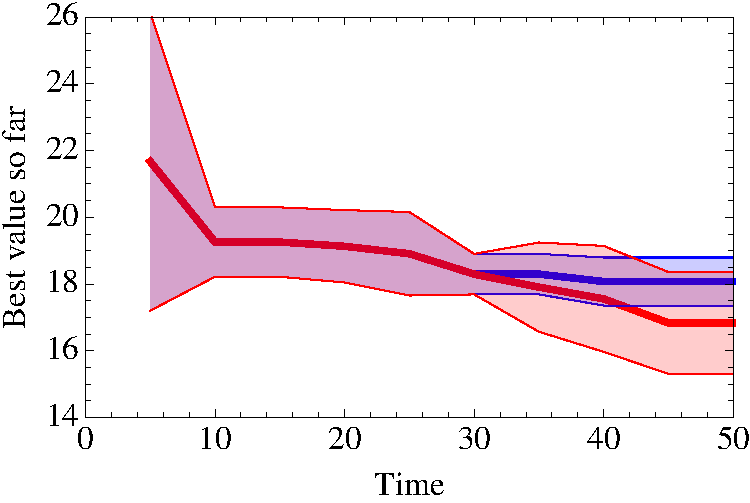
\includegraphics[scale=.39]{../nips2011paper/figures/bostonHousing.pdf}
\vs{3}
\captionof{figure}{\label{fig:boston}
  GP optimizing neural network hyper-parameters on the Boston
  Housing regression task. Shown: best minimum found so far
  every 5 iterations, against time. Red = GP, Blue = Random. Shaded
  areas = one-sigma error bars.
  }
\end{center}
\end{minipage}
%}
&
%\fbox{
\hspace*{6mm}\begin{minipage}{0.45\linewidth}
    \begin{center}
    \begin{tabular}{lll}
                & {\bf convex} & {\bf MRBI} \\
        \hline
        GM & {\bf 14.13} $ \pm 0.30$ \% & {\bf 44.55} $ \pm 0.44$\%   \\
        GP & $ 16.70 \pm 0.32$\% &  $ 47.08\pm 0.44 $\% \\
        Manual & $18.63 \pm 0.34$\%  &  $47.39 \pm 0.44$\%  \\
        Random &  $ 18.97\pm 0.34$ \%  & $46.22 \pm 0.44$\% \\
        \hline
    \end{tabular}
    \end{center}
    \caption{The test set classification error of the best model
    found by each search algorithm on each problem.
    Each search algorithm was allowed up to 200 trials.
    The manual searches used 82 trials for {\bf convex}
    and 27 trials ``MNIST rotated background images'' ({\bf MRBI}).
    \label{tbl:testerr}
    }
\end{minipage}
%}
\end{tabular}
\end{center}
\vs{6}
\end{table}


The GP and GM algorithms are quite general, not DBN-specific.
They apply to a broad range of configuration problems involving
fixed or variable numbers of parameters that each might be discrete, ordinal, or continuous.
This paper describes how the \hyperopt\ software package allows them to be used in new optimization problems,
and how to try new optimization strategies on problems such as DBN configuation..



\Bs
\section{Sequential Model-based Global Optimization}
\as
\label{sec:smbo}

The GM and GP algorithms presented in \cite{nipspaper} fit into the framework
of Sequential Model-Based Global Optimization (SMBO).
SMBO algorithms have been used in many applications
where evaluation of the fitness function is expensive~\citep{hutter:2009,hutter+hoos+leyton+brown:2011}.
In an application where the true fitness function
$f:\cX\rightarrow \mathbb{R}$ is costly to evaluate,
model-based algorithms approximate $f$
with a surrogate that is cheaper to evaluate.
Typically the inner loop in an SMBO algorithm is the numerical optimization of this surrogate,
or some transformation of the surrogate.
The point $x^*$ that maximizes the surrogate (or its transformation) becomes the proposal
for where the true function $f$ should be evaluated.
This active-learning-like algorithm template is summarized in Figure~\ref{f:genericAlgo}.

%\setlength{\algowidth}{0.95\textwidth}
\begin{figure}[!ht]
\vs{2}
\centerline{
\begin{algorithm}{$\Algo{SMBO}\big(f,M_0, T,S \big)$}
\Aitem $\cH \setto \emptyset$,
\Aitem For $t \setto 1$ \To $T$,
\Aitem \label{ai:candidate}\mt Generate candidate $x^*$ by optimizing
criterion $S$ on model $M_{t-1}$,
\Aitem \mt Evaluate $f(x^*)$, \mt \algoremark{Expensive step}
\Aitem \mt $\cH \setto \cH \cup (x^*,f(x^*))$,
\Aitem \mt \label{ai:update} Fit a new model $M_t$ to $\cH$.
\Aitem \Return $\cH$
\end{algorithm}
}
\vs{2}
\caption{The pseudo-code of a generic Sequential Model-Based
  Optimization algorithm.}
\label{f:genericAlgo}
\vs{0}
\end{figure}

SMBO algorithms are differentiated in how they approximate $f$,
and in the criterion that they optimize to get $x^*$.
\citet{nipspaper} looked at two SMBO algorithms for optimizing hyper-parameters:
one based on Gaussian Process regression (GP) for modeling $P(y=f(x)|x)$
and one based on a simple non-parametric graphical model (GM) of the
joint distribution $P(x,y=f(x))$.
Both algorithms optimized the criterion of expected improvement (EI) in
some surrogate to identify the proposal $x^*$ in the SMBO template.

\subsection{Parallelizing Sequential Optimization}

SMBO algorithms are fundamentally {\em sequential} rather than parallel.
However, when there is enough data to warrant a complex algorithm (requiring automatic configuration)
it also typically takes a lot of CPU time (tens or hundreds of minutes) to use all of that data in testing that algorithm.
Researchers in machine learning are accustomed to using a compute cluster
to optimize hyper-parameters because they can parallelize those calculations.
It is of little practical use to use a sequential algorithm that cannot outperform a cluster
in terms of quality of solution as a function of wall time.
We need the optimization algorithm to parellelize the evaluations on line 4 of
Figure~\ref{f:genericAlgo}.

\hyperopt\ parallelizes sequential optimization by running the evaluations of line 4 asynchronously,
and updating the database of results ($\cH$) asynchronously as those evaluation jobs complete.
While the evaluation of the $t^{\mathrm{th}}$ proposal is in progress,
it is marked temporarily as having a constant, disappointing score (the {\em constant liar} approach, \cite{ginsbourger+leriche+carraro:2010}).
A disapponting score prevents subsequent proposals $t+\tau$ from exploring nearby locations redundantly.


\subsection{Major Implementation Components}

Our implementation of asynchronous SMBO employs a client-server architecture.
The server is a standard MongoDB.
MongoDB is used both to track the state of the experiment $\cH$ and as a
message board for more general inter-process communication between the clients.
The clients are Python programs implemented in the \hyperopt\ package.
Two scripts are used
to conduct a distributed asynchronous optimization: \mongoworker\ and \mongosearch.


\begin{description}
\item[\mongoworker] - worker loop\\
    Called from the command-line with options to connect to a particular mongo server,
    it polls the server for a new candidate $h$ in $\cH$ and evaluates it.
\item[\mongosearch] - server loop\\
    Called from the command-line with options to connect to a particular mongo server,
    it polls the server and inserts a new candidate into $\cH$ whenever the existing ones
    have all been taken by worker clients.
\end{description}


The \mongoworker\ script polls the mongo server and
atomically fetches an un-started candidate $h$ from $\cH$, which is a JSON (JavaScript Object Notation) document.
It uses a field in $h$ to identify the python function $f$ that is to be used to evaluate the candidate.
It extracts the candidate configuration subdocument ($C$).
It constructs a control object via which the evaluation function can communicate with mongo and other processes ($R$).
Finally it executes a sub-process that calls $f(C, R)$.
When $f$ returns, the subprocess marks $h$ as being complete (or failed with an error).
The \mongoworker\ script is meant to be launched using existing cluster dispatching software such as Torque, PBS, or SGE.
A single experiment can draw on \mongoworker\ scripts running on multiple networks and clusters,
the bandwidth requirement for communication between \mongoworker\ and \mongo\ can be very low.

The \mongosearch\ script requires command-line arguments specifying
(a) the optimization algorithm and
(b) the evaluation function.
The script polls the mongo server
and when there are zero new candidates in $\cH$ it appeals to a plug-in (indicated by the command-line arguments)
to suggest a new candidate.
The plug-in makes a suggestion based on the state, the configuration, and the evaluation result of each $h \in \cH$.
The state of each $h$ is either ``new'', ``running'', ``finished successfully'', or ``finished in error''.
The \mongosearch\ script inserts that candidate into $\cH$, where it will be picked up by an idle \mongoworker.
The \mongoworker\ and \mongosearch\ script are independent clients from the operating system's perspective:
either one can be killed and restarted without disrupting the other.
\mongosearch saves its state to the MongoDB if it is killed with CTRL-C, so that it can be resumed later.

\subsection{Using hyperopt to optimize a new function}

To optimize a new function with \hyperopt, implement the evaluation function $f$ as a {\tt Bandit} subclass.
In \hyperopt, a Bandit carries two pieces of information:
\begin{itemize}
    \item a callable function (corresponding to $f$ in Figure~\ref{f:genericAlgo})
    \item a prior over the configuration argument to $f$ (see Figure~\ref{f:htdict}).
\end{itemize}
The callable function is simply a class method or static method of your bandit subclass.
The prior over configuration arguments can be specified with the stochastic expression
language defined within \hyperopt\ (see Figure~\ref{f:htdict} for an example).
This language is makes it easy to express broad, simple priors.
it is possible to write a more complicated prior distributions over the configuration space
by writing a stochastic Theano program.\footnote{
Stochastic Theano programs implemented with MonteTheano:
\url{http://www.github.com/jaberg/MonteTheano}}
Both of these methods provide a graphical description of the
configuration space to an optimization algorithm.

\begin{figure}
\begin{minipage}{\textwidth}
\small
\begin{verbatim}
    rdict(
        "preprocessing", one_of(
            rdict(
                "kind", "raw"),
            rdict(
                "kind", "zca",
                "energy", uniform(low=0.5, high=1.0))),
        "dataset_name", "MNIST",
        "seed", one_of(5, 6, 7, 8),
        "batchsize", one_of(1, 20, 100),
        "lr", lognormal(mu=log(.01), sigma=3),
        "lr_anneal_start", ceil_lognormal(mu=log(1000), sigma=2),
        "l2_penalty", one_of(0, lognormal(mu=log(1.0e-6), sigma=3)),
        "n_hid", ceil_lognormal(mu=log(512), sigma=3, round=16))
\end{verbatim}
\end{minipage}
\caption{Specification of a search space using random dictionaries
({\tt \small rdict}), random choices ({\tt \small one\_of}), and random numbers ({\tt \small uniform},
{\tt \small lognormal}, {\tt \small ceil\_lognormal}).
Optimization algorithms in \hyperopt\ inspect this data structure to
draw random samples, infer posteriors, and define kernel functions in the configuration space.
}
\label{f:htdict}
\end{figure}

The structure of the configuration description can have an impact on search algorithms.
For example, Figure~\ref{f:htdict} uses a nested random variable to define the energy of the ZCA preprocessing option.
We could express exactly the same prior if preprocessing were defined as
{\tt one\_of("raw", "zca")} and {\tt "energy"} were promoted to a top-level configuration field.
However, these two expressions of the prior would lead to different kernels in the GP optimization algorithm.
In the former case energy would not enter into the distance between trials with "raw" preprocessing.
In the latter case, it would.
It is our hope that a single description of a configuration space suffices to get the best performance from all optimization algorithms.


\subsection{Optimization Algorithms}

\hyperopt\ provides three optimization algorithms:
random search,
the GM algorithm from~\cite{nipspaper},
and the GP algorithm from~\cite{nipspaper}.
More algorithms are planned by the authors,
and contributions from other researchers are welcome.

Optimization algorithms should inherit from the {\tt BanditAlgo} (or {\tt TheanoBanditAlgo}) base classes.
Those classes have a virtual method {\tt suggest} (or {\tt theano\_suggest} that derived classes must implement.
The details of how those functions should be implemented are provided in the code and documentation online.
Essentially those functions accept the current state of $\cH$ as an argument
and return some number of promising candidates
$x^*$ for \mongosearch\ to insert in the database.

\subsection{Other notable resources}

\hyperopt\ also includes:
\begin{itemize}
\item \mongoshow\ - a script for rapid visualization of the state of an experiment.
It can display a scatterplot of scores against time,
or against the various hyper-parameters of the configuration space.
It serves additionally as a starting point for custom visualization code.
\item {\tt search} - a script for serial-mode evaluation that works without MongoDB.
\item Simple inexpensive bandits for testing optimization algorithms.
\end{itemize}


\section{Conclusion}

Bayesian optimization and sequential model-based optimization represent
promising approaches to hyper-parameter optimization.
This paper has introduced \hyperopt, an open source package for
distributed hyper-parameter
optimization. It implements the algorithms of \cite{nipspaper},
and provides extensible platform for future work.
For more information, please follow the development of \hyperopt\ online at
\url{http://www.github.com/jaberg/hyperopt}.

\small
\bibliographystyle{unsrt}
\bibliography{strings,strings-short,strings-shorter,jb,hyperoptim}

\end{document}


\Bs
\subsection{Gaussian Processes}
\as
\label{ss:GPs}
Gaussian Processes (GPs, \cite{RaWi06}) are priors over functions that are
{\it closed under sampling}, which means that if the prior
distribution of $f$ is believed to be a GP, the conditional
distribution of $f$ knowing a sample $(x_i,f(x_i))_{i=1}^n$ of its
values is still a GP, whose parameters can be obtained
analytically. This, and the fact that GPs provide an assessment of
prediction uncertainty incorporating the effect of data scarcity, 
makes GPs an elegant candidate for the surrogate
model $M_t$ of the algorithm in Figure \ref{f:genericAlgo}, in which
step \ref{ai:update} is carried out easily. The idea of Gaussian
Process-based global optimization dates back to the 70's
\cite{MoTiZi78}. We first review a few notations and concepts on GPs,
following \cite{RaWi06} and then consider several ways of implementing
step \ref{ai:candidate} of SMBO.

Let $k$ be a positive definite kernel on the input space
$\mathcal{X}$. Under a $\text{GP}(0,k)$ prior, the distribution of any
vector of function values ${\bf y}=(f(x_1), ... , f(x_n))^{T}$ is a
multivariate Gaussian ${\bf y} \sim \mathcal{N}(0,K)$, where 
$K_{ij}:=k(x_i,x_j)$. GPs with
generic mean functions can in principle be used, but it is simpler
and sufficient for our purposes to only consider zero mean processes.
We do this by
centering the function values in the considered data sets, as modelling
nonconstant trends in the GP mean can lead to
overconfident behavior of SMBO in unexplored regions \cite{GiDuBaCaRo09}.

We already mentioned that the GP prior is closed under sampling:
given a prior $p(f) \sim \text{GP}(0,k)$ over functions and a set of samples
$\mathcal{D}:=\big\{(x_i,f(x_i)) ; 1\leq i\leq n\big\}$, the posterior
$p(f\vert\mathcal{D})$ is also a GP with mean $
\widetilde{m}(x) = k(x,{\bf x})K^{-1}{\bf y}$ and covariance function
$\widetilde{k}(x,x') = k(x,x')-k(x,{\bf x})K^{-1}k({\bf x},x')$.


Predictions about the function value $f(x)$ at a test point $x$
are then straightforward, since according to the posterior, $f(x)$
has distribution $\mathcal{N}(\widetilde{m}(x),\widetilde{k}(x,x)).$ Note that
the posterior variance at training points vanishes, as the
observations are noiseless. Additive homoscedastic (input-independent)
Gaussian noise can however be handled easily \cite{RaWi06}.

Now step \ref{ai:candidate} of the SMBO algorithm in Figure
\ref{f:genericAlgo} is usually defined itself as an optimization
task, where an auxiliary criterion $S(x)$ reflecting the interest of
evaluating $f$ at a new point $x\in\cX$ is maximized. Various such
auxiliary criteria have been suggested: among which maximizing the
Probability of Improvement and Expected Improvement (a good review can
be found in \cite{Jon01}), minimizing the Conditional Entropy of the
Minimizer \cite{ViVaWa06}, or recently, a bandit-based criterion
\cite{SrKrKaSe10}. The most widespread remains however
the so-called Expected Improvement criterion (EI, \cite{Jon01}).

\Bss
\subsection{The Expected Improvement criterion}
\ass

Assume we want to minimize an unknown fitness function $f$ that has already
been evaluated at $n$ points from $\mathcal{D}:=\{(x_i,f(x_i)) ; 1\leq
i\leq n\}.$ Assume you have a model $p(y\vert x,\cF_n)$ of $f$ where
$\mathcal{F}_n$ is the $\sigma$-algebra generated by the previous
fitness evaluations summarized in $\mathcal{D}$. The EI strategy
defines the next point $x_{n+1}$ to be
evaluated as the point where the expected improvement over 
%the currently best minimum $m_n:=\min_i f(x_i)$ 
a user-defined value $y^*\in\mathbb{R}$ is the highest. The EI
criterion then reads
\begin{equation}
\vs{.5}
\text{EI}_{y^*}(x):=\mathbb{E}\big(\max(y^*-f(x),0)\vert \mathcal{F}_n\big).
\label{e:EI}
\vs{.5}
\end{equation}
Recall from Section \ref{ss:GPs} that under a GP model on $f$, we have 
$$p(y\vert x,\cF_n) = \cN(\widetilde{m}(x),\widetilde{\sigma}(x)^2),$$ 
where $\tilde\sigma(x) = \tilde{k}(x,x)$. A direct computation then yields
\begin{equation}\label{e:EIunderGP}
\vs{.5}
 \text{EI}_{y^*}(x)=\widetilde{\sigma}(x)\big(u(x)\Phi(u(x))+\phi(u(x))\big),
\vs{.5}
\end{equation}
where $u(x)=(y^*-\widetilde{m}(x))/\widetilde{\sigma}(x)$, and $\Phi$ and
$\phi$ denote the cdf and pdf of the $\mathcal{N}(0,1)$ distribution,
respectively. This alternative definition makes it easier to remark that EI
encapsulates a compromise between regions where the mean function is
close to or better than the best value obtained so far and
under-explored regions
where the uncertainty is high. The next two subsections describe two different
algorithms that use the EI criterion to propose candidates in step
\ref{ai:candidate} of SMBO.

\Bss
\subsection{Optimizing the EI criterion with Evolutionary Algorithms}
\ass
\label{ss:ea}

We put here a GP model on $f$ and set $y^*$ to the best value found so far $y^*=m_n:=\min\{
f(x_i),1\leq i\leq n\}$. Traditionally, EI is optimized in a greedy fashion, by putting
either a grid over $\cX$ or using Latin Hypercube sampling \cite{ViVaWa06},
depending on the dimension of $\cX$ and the budget allowed for this
auxiliary task. However, \eqref{e:EIunderGP}
also gives some information on the landscape of the EI criterion, that can be
used to derive Evolutionary Algorithms specifically designed to
optimize EI \citep{BaKe10}: 1) it is
always non-negative and zero at training points from $\mathcal{D}$, 2) it
inherits the smoothness of the kernel $k$, which is
in practice often at least once differentiable, and noticeably, 3) the
EI criterion is likely to be highly multi-modal, especially as the number of
training points increases. 

The EI function is usually optimized with an exhaustive grid search
over the input space, or an equivalent Latin Hypercube search for
higher dimensions. The authors of \cite{BaKe10} used the
preceding remarks on the landscape of EI to design an evolutionary
algorithm with mixture search, specifically aimed at optimizing EI,
that is shown to outperform exhaustive search for a given budget in EI
evaluations. We borrow here their approach and go one step further. We keep the
Estimation of Distribution (EDA, \cite{LaLo01}) approach on the discrete
part of our input space (categorical and
discrete hyper-parameters), where we sample candidate points according
to binomial distributions, while we use the Covariance Matrix Adaptation -
Evolution Strategy (CMA-ES, \cite{Han06}) for the remaining part of
our input space (continuous hyper-parameters). CMA-ES is a
state-of-the-art evolutionary algorithm for optimization on continuous
domains, which has been shown to outperform the Gaussian search
EDA. We do not take on the use
of mixtures in \cite{BaKe10}, but rather restart the local searches
several times, starting from promising places. The authors of
\cite{BaKe10} suggest
the latter can be defined as centers of simplices obtained through
tessellations of the set of points where the fitness function has
already been evaluated (the ``training set''), but as our task often means
working in more than 10 dimensions, these tessellations are too
expensive to obtain, thus we start each local search at the center of mass of a
simplex with vertices randomly picked among the training points.

Finally, we remark that all hyper-parameters are not relevant for each
point. A DBN with only
one hidden layer e.g. does not have parameters associated to its second or
third layer. Thus it is not enough to place one GP over the entire
space of hyper-parameters. We chose to group the hyper-parameters by
common use in a tree-like fashion and place different independent GPs
over each group. As an example, for DBNs, this means placing one GP over common
hyper-parameters, including categorical parameters that indicate what
are the {\it conditional} groups to consider, three GPs on the
parameters corresponding to each of the three layers, and a few 1D GPs
over individual conditional hyper-parameters, like ZCA
energy.

\Bss
\subsection{Another approach at EI optimization: sampling from a
  tree-structured model}
\label{ss:tree}
\ass

Anticipating that our hyper-parameter optimization tasks will mean high
dimensions and small fitness evaluation budgets, we now turn to
an alternate way to encode step \ref{ai:candidate} of the
SMBO algorithm shown in Figure \ref{f:genericAlgo} that not does
assume a GP model over $f$, but
still relies on optimizing \ref{e:EI}, with the intent of being less
sensible to the uncertainty on $f$ in unexplored regions, thus
favoring exploitation over exploration. We compare this approach and
the Evolutionary Algorithm approach of Subsection \ref{ss:ea} in Section \ref{sec:exp}.

We first model the joint distribution $p(x,y)$ between the inputs
$x\in\cX$ and the values $y\in\mathbb{R}$ of $f$. We assume that
$p(x,y)$ factorizes in the following tree-structured model, which is
natural in the case of Deep Neural Networks:
\begin{eqnarray}
    p(x,y) &\propto& p(y) p(x\vert y) p(y) p(\text{pre-processing hyper-parameters}|y) \nonumber\\
     & & p(\text{use hidden layer}|y) p(\text{hidden layer
      hyper-parameters}|\text{use hidden layer}, y) \label{e:factor}.
\end{eqnarray}
Recall that we assume having already evaluated $f$ at $n$ points $\mathcal{D}:=\{(x_i,f(x_i)) ; 1\leq
i\leq n\}$. We model $p(y)$ with $q(y)$\footnote{For ease of notation, we will drop any conditioning on
$\mathcal{D}$ or $\cF_n$ in the following notations.}, a Parzen window
model fit to the data
$\{y_1,...,y_n\}$. Now, given a threshold $y^*$ under
which you consider there's an improvement, there
are two regions of interest: $G_{y^*} := \{(x,f(x))\in\cX\times\mathbb{R}: f(x) \geq y^*\}\text{
  and  }L_{y^*} = \{(x,f(x))\in\cX\times\mathbb{R}: y<y^*\}$.
 We thus fit $p(x\vert y)$ with two tree-structured
distributions $\ell(x)$ and $g(x)$ of $x$ given respectively $y<y^*$ and
$y\geq y^*$. Each of these two distributions has the same
factorization given in \eqref{e:factor}, which reflects the natural
generative process of the
parameters of a multi-layer model: first choose parameters related to
the pre-processing of the data,
then choose parameters related to the first layer of the model (and
second, third, and so on), and finally choose parameters related to
the strategy for classifying features. Now, we turn to finding an
equivalent of \eqref{e:EIunderGP} under this new model:
\begin{align}
\vs{.5}
    \mathrm{EI}_{y^*}(x)
    = \int_{-\infty}^{y^*} (y^* - y)p(y|x) dy
    \approx \int_{-\infty}^{y^*} (y^* - y) \frac{p(x|y)q(y)}{p(x)}
    dy
\vs{.5}
\end{align}
Now if we denote by $\gamma = p(y<y^*)\approx q(y<y^*)$, remark that 
$
%\vs{.5}
p(x) \approx \int_\mathbb{R} p(x\vert y) q(y) dy = \gamma \ell(x) +
(1-\gamma) g(x),
%\vs{.5}
$
and
\begin{eqnarray}
\vs{.5}
\int_{-\infty}^{y^*} (y^* - y) p(x|y)q(y) dy &\approx&
\ell(x)\int_{-\infty}^{y^*} (y^* - y) q(y) dy\nonumber= \gamma y^*\ell(x) - \ell(x)\int_{-\infty}^{y^*} q(y)dy,
\vs{.5}
\end{eqnarray}
so that finally
%\begin{eqnarray*}
%\vs{.5}
$
EI_{y^*}(x) \approx \frac{\gamma y^*\ell(x) - \ell(x)\int_{-\infty}^{y^*} q(y)dy}{\gamma \ell(x) +
(1-\gamma) g(x)}
\propto \left( \gamma + \frac{g(x)}{\ell(x)}(1-\gamma)\right)^{-1}.
$
%\vs{.5}
%\end{eqnarray*}
This last expression shows that to maximize improvement we would like
points $x$ with high probability under $\ell(x)$ and low probability
under $g(x)$. The tree-structured form of $\ell$ and $g$ makes it easy to draw many candidates according to $\ell$ and evaluate them according to $g$;
together these steps reveal a candidate with high EI. Note finally
that the choice of the quantile $\gamma\in[0,1]$ is left free to the user.

\begin{table}
\vs{4}
    \caption{Distribution over DBN hyper-parameters for random sampling.
    Options separated by ``or''  such as pre-processing (and including the random seed) are weighted equally.
    Symbol $U$ means uniform, $\mathcal{N}$ means Gaussian-distributed, and $\log U$ means uniformly distributed in the log-domain.
    CD (also known as CD-1) stands for contrastive divergence, the algorithm used to initialize the layer parameters of the DBN.
    %and the distribution used by the \algorandom\ algorithm.
    }
    \label{tbl:dbnprior}
    \centering
    \begin{tabular}{llp{.1in}ll}
        \multicolumn{2}{c}{{\bf Whole model}} & & \multicolumn{2}{c}{\bf Per-layer} \\
        Parameter & Prior & & Parameter & Prior \\
        \hline
        pre-processing & raw or ZCA & & n. hidden units & $\log U(128, 4096)$\\
        ZCA energy & $U(.5, 1)$ & & $W$ init & $U(-a,a)$ or $\mathcal{N}(0, a^2)$ \\
        random seed & 5 choices & & $a$ & algo A or B (see text)\\
        classifier learn rate & $\log U(0.001, 10)$ & & algo A coef& $U(.2,2)$\\
        classifier anneal start & $\log U(100, 10^4)$ & & CD epochs & $\log U(1, 10^4)$\\
        classifier $\ell_2$-penalty & 0 or $\log U(10^{-7}, 10^{-4})$ & & CD learn rate & $\log U(10^{-4},1)$ \\
        n. layers & 1 to 3 & & CD anneal start & $\log U(10, 10^4)$ \\
        batch size & 20 or 100 & & CD sample data & yes or no \\
        \hline
    \end{tabular}
\vs{4}
\end{table}

\Bss
\subsection{Parallelizing searches}
\ass

To allow the use of parallel computing units and waste as little time
as possible waiting for an evaluation to finish, both instances of
SMBO described in Sections \ref{ss:ea} and \ref{ss:tree} were used to
predict up to five steps in
the future. For the GP approach of Section \ref{ss:ea}, the so-called
{\it constant liar} approach was used: each time a candidate point $x$
is proposed, a fake fitness function equal to the mean of the $y$'s
within the training set $\mathcal{D}$ is assigned to him, and the next
candidate results of optimizing this augmented model. For the
graphical model-based approach (GM) of Section \ref{ss:tree}, we ignored recently proposed points
and relied on the stochasticity of draws from $\ell(x)$ to provide different candidates
from one iteration to the next.

\Bss
\subsection{Updating the GM algorithm's density model}
\ass

For the first few trials (a hyper-parameter of the GM),
the GM algorithm drew from the initial distribution defined in Table~\ref{tbl:dbnprior}.
After the initial random sampling, the GM algorithm switches to the use of EI based on $l(x)$ and $g(x)$.
For discrete hyper-parameters, $l(x_i=C)$ and $g(x_i=C)$ were proportional to $1+count(C)$.
For continuous hyper-parameters, $l(x_i=a)$ and $g(x_i=a)$
were a uniform prior over the whole domain with the strength of one observation,
plus Gaussians as per the Parzen Windows algorithm.
The width of each Gaussian was set independently according to a heuristic:
its standard deviation (width) was chosen to be the
greater of the distances to the left and right neighbor, 
where the lower and upper bounds of the uniform could also be considered to be neighbors.
The mixture defined this way could technically grow beyond the initial uniform bounds,
and we allowed this in all cases except the lower bound of log-uniform distributions.


\Bs
\section{Experimental Setup}
\label{sec:exp}
%\as
%\subsection{Validating surrogate modelling on the Boston Housing dataset}
%\ass
We first validated the use of surrogate optimization by comparing our
GP approach of Section \ref{ss:ea} with random sampling on the Boston
Housing dataset, a regression task with 506 points made of 13 scaled
input variables and a scalar regressed output. We trained a
Multi-Layer Perceptron (MLP) with 10 hyper-parameters,
including learning rate, $L^1$ and $L^2$ penalties, size of hidden
layer, number of iterations, whether a PCA preprocessing was to be
applied, whose energy was the only conditional hyper-parameter~\citep{Bis95}. Our
results are depicted in Figure~\ref{fig:boston}. The first 30 iterations
were made using random sampling, while from the 30th on, we
differentiated the random samples from the GP approach trained on the
updated history. The experiment was repeated 20 times. Although the
number of points is particularly small compared to the dimensionality,
the surrogate modelling approach finds noticeably better points than
random, which justifies trying to apply our two SMBO approaches on
more ambitious tasks and datasets. 

The GP and GM algorithms were applied to the problem of optimizing DBN performance on the {\bf convex} and {\bf MRBI} datasets.
For the GP-based algorithm, we allowed 3 random restarts to the CMA+ES algorithm per proposal $x^*$,
and up to 500 iterations of conjugate gradient method in fitting the
length scales of the GP. In the GP method, the squared
exponential kernel \cite{RaWi06} was used for every node. The CMA-ES part of GPs
dealt with boundaries using a penalty method, the binomial sampling
part dealt with it by nature. After 200 trials, the prediction of a point $x^*$ using this GP took around 150 seconds.

For the GM-based algorithm, we choose $\gamma=0.15$ and picked the best among 100 candidates drawn from $l(x)$
on each iteration as the proposal $x^*$.  After 200 trials, the prediction of a point $x^*$ using this GM algorithm
took around 10 seconds.
GM was allowed to grow past the initial bounds used with for
random sampling in the course of optimization, whereas the GP (and random search)
was restricted (due simply to implementation details) to stay within the initial bounds
throughout the course of optimization.
For comparison, we also evaluated many randomly-chosen trials from the initial 
sampling distribution (457 and 361 from {\bf convex} and {\bf MRBI} respectively).

Runtime per trial was limited to 1 hour of GPU computation regardless of whether execution was on a GTX 285, 470, 480, or 580. The difference in speed between the slowest and fastest machine was roughly two-fold in theory, but the actual efficiency of computation depended also on the load of the machine and the configuration of the problem (the relative speed of the different cards is different in different hyper-parameter configurations).
With the parallel evaluation of up to five proposals from the GP and GM algorithms, each experiment took about 24 hours of wall time using five GPUs.

\begin{figure}
% /home/bergstra/cvs/hyperopt/hyperopt/dbn.py plot_histories mongo://localhost:20111/dbn_%s_%s/jobs gp3,gm convex 0 2000
  \vs{0}
    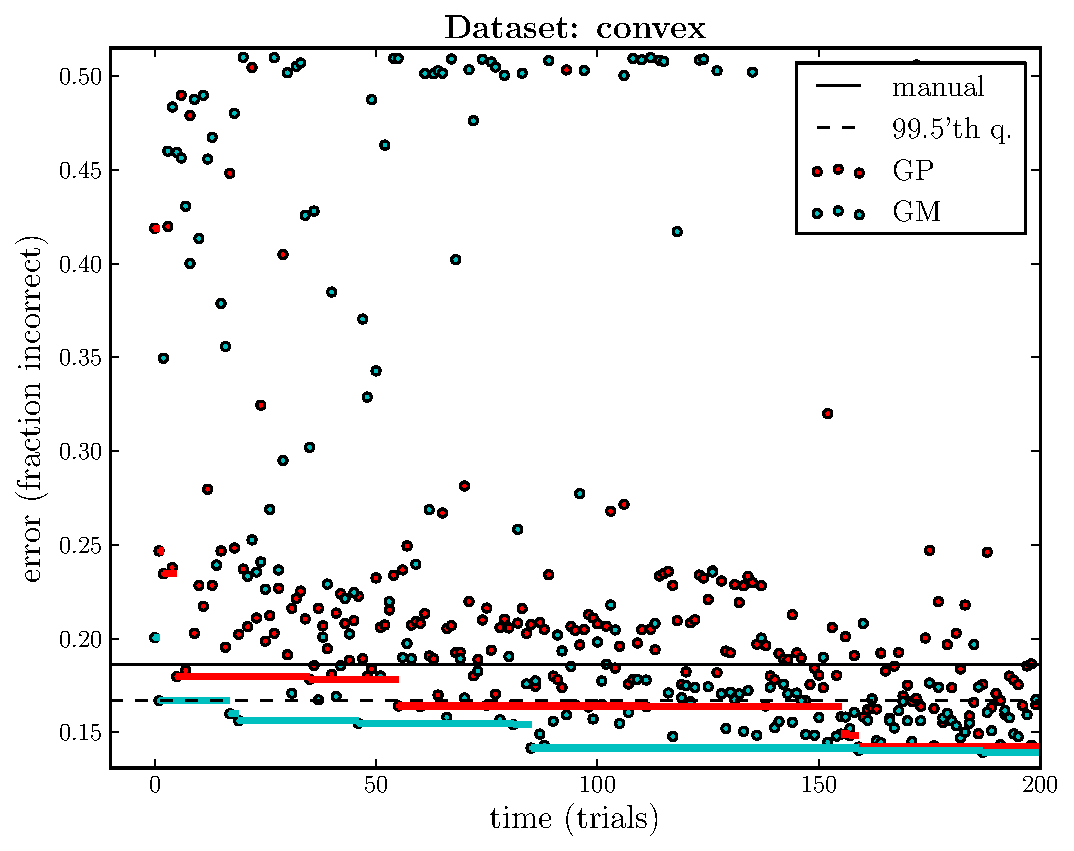
\includegraphics[scale=.39]{../nips2011paper/figures/plot_histories_gp3,gm_convex}
    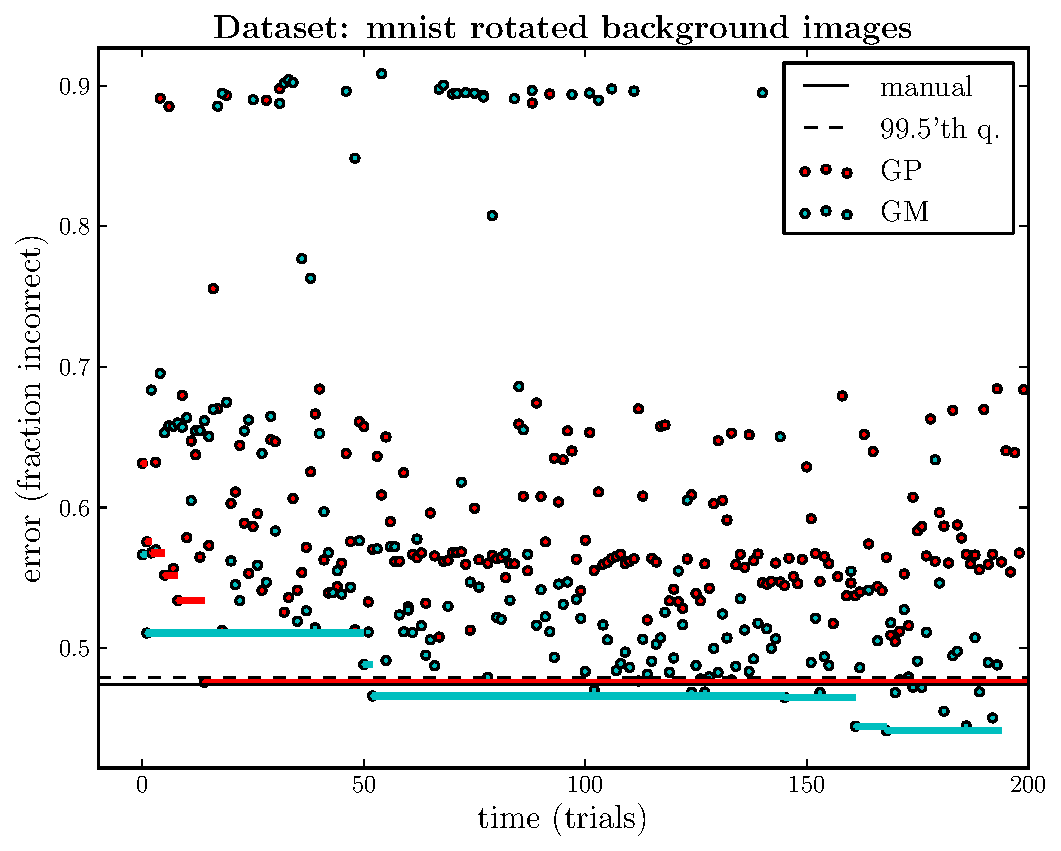
\includegraphics[scale=.39]{../nips2011paper/figures/plot_histories_gp3,gm_mnist_rotated_background_images}
  \vs{6}
% /home/bergstra/cvs/hyperopt/hyperopt/dbn.py plot_histories mongo://localhost:20111/dbn_%s_%s/jobs gp3,gm mnist_rotated_backgound_images 0 2000
    \caption{Efficiency of Gaussian Process-based (GP) and graphical
    model-based (GM) sequential optimization algorithms on the task of optimizing the validation set performance of a DBN of up to three layers on the {\bf convex} task (left) and the {\bf MRBI} task (right).
    The dots are the elements of the trajectory $\cH$ produced by each SMBO algorithm.
    The solid coloured lines are the validation set accuracy of the best trial found before each point in time.
    Both the GM and GP algorithms make significant advances from their random
    initial conditions, and substantially outperform the manual and random
    search methods. A 95\% confidence interval
    about the best validation means on the {\bf convex} task extends 0.018 above and below each point,
    and on the {\bf MRBI} task extends 0.021 above and below each point.
    The solid black line is the test set accuracy obtained by domain experts using a combination
    of grid search and manual search~\citep{Larochelle+etal:2007}.
    The dashed line is the 99.5\% quantile of validation performance found among trials sampled from our prior distribution (see Table~\ref{tbl:dbnprior}),
    estimated from 457 and 361 random trials on the two datasets respectively.
    % convex has n=1500 validation points
    % best scores have Bernoulli param p = 0.15
    % variance is 1.96 sqrt(p * (1-p)/n) = 0.018%
    % MRBI has n=2000 validation points, p=.45
    }
  \vs{4}
    \label{fig:H}
\end{figure}


\Bs
\section{Discussion}
\label{sec:discussion}
\as

The trajectories ($\cH$) constructed by each algorithm up to 200 steps are illustrated in Figure~\ref{fig:H}.
On the {\bf convex} dataset both algorithms converged to a validation score of 13\% error, which is significantly better than both manual search (19\% on test) and random search with 200 trials (17\%).
On the {\bf MRBI} dataset, each of manual search, random search with 200 trials, and the GP algorithm achieved the same result (47\% error), while the GM algorithm found a new best result (44\% error).
The generalization scores of the best models found using these algorithms and others are listed in Table~\ref{tbl:testerr}. The models found by the GM algorithm in particular are better than previously found ones, on both datasets, on out-of-sample data as well.

%Look at some of the scatter plots - which parameters turned out to be most important?

%We added the possibility of ZCA pre-processing, did it help any?

%What about depth - what do the optimization algorithms choose for the number of layers?

%What is a good termination condition for these sequential algorithms?

The fact that the GM algorithm outperforms the GP algorithm in these problems suggests either
that 1) the graphical model factorization of $P(y|x)$ is more accurate than the Gaussian process,
or perhaps 2) conversely that the exploration induced by the graphical
model's lack of accuracy is actually a good thing for search, or
finally 3) that given the GP spends too much time exploring the space
in our regime of small evaluation budget and high dimension. The
latter cause might express the need for more ``aggressive'' criteria
than EI, i.e. switching ``earlier'' than EI to an exploitation mode.  
More (computationally expensive) experiments are necessary to establish a relative ordering between them
on these particular datasets.
What is more conclusive is that all four SMBO runs matched or exceeded both random search and human search,
which are the current state of the art for hyper-parameter optimization.
%The difference in their ordering could be a statistical anomaly
% - let the reviewer point that one out, and hopefully we'll be ready with
%   error bars by the time the review period comes along.

The GP and GM algorithms work well in both of these settings,
but there are certainly settings in which these algorithms would not be expected to do well.
Both algorithms depend on an accurate model of $P(y|x)$ -- the worse is the surrogate model,
the worse are these sequential algorithms.  It is possible to do worse than random sampling
with a badly chosen model for $P(y|x)$. Obviously, if the search problem is too easy, then these algorithms will fail to outperform random search.
For example, if 30 trials from the prior can be expected to find a near-optimal solution then the problem will already be solved by the time the EI criterion is even used.
Another setting in which these algorithms can fail to outperform random search
is in the case of needle-in-haystack type search problems. Sequential optimization algorithms work by leveraging structure in observed $(x,y)$ pairs,
so while no structure is evident these algorithms are equivalent to random.

\Bs
\section{Conclusion}
\label{sec:conclusion}
\as

This paper has introduced two sequential hyper-parameter optimization algorithms,
and shown them to meet or exceed human performance and the performance of a brute-force random search
in two difficult hyper-parameter optimization tasks involving DBNs.
We relax standard constraints (e.g. equal layer sizes at all layers) on the search space,
and fall back on a more natural hyper-parameter space of 32 variables
(including both discrete and continuous variables)
in which many variables are sometimes irrelevant,
depending on the value of other parameters (e.g. the number of layers).
In this 32-dimensional search problem,
the GM algorithm presented here has uncovered new best results on both of these datasets that are significantly better than what DBNs were previously believed to achieve.
Moreover, the GP and GM algorithms are practical: the optimization for each dataset was done in just 24 hours using five GPU processors.
Although our results are only for DBNs, our methods are quite general, and extend naturally (as far as we know) to any hyper-parameter optimization problem in which the hyper-parameters are drawn from a measurable set.

We hope that the machine learning community can start to treat the
hyper-parameter optimization strategy as an interesting and important component of a learning algorithm.
The question of ``How well does a DBN do on the {\bf convex} task?'' is not in fact very well-defined --
different approaches to hyper-parameter optimization will give different answers.
Algorithmic approaches to hyper-parameter optimization make machine learning results easier to disseminate, reproduce, and transfer to other domains.

Finally, powerful hyper-parameter optimization algorithms broaden the horizon of models that can realistically be studied; researchers need no longer to restrict themselves to systems of a few variables that can readily be tuned by hand.


%It is important to include the hyper-parameter optimization algorithm in the specification of a learning algorithm.
%Perhaps there is a hyper-parameter configuration that leads a DBN to perfect performance, that does not mean that DBNs simply have 0\% error! We must include the procedure for finding that configuration.
%




\iffalse
Vincent+etal:2010 used it. They found the SDA3 model superior to DBN3 on both datasets.
SDA3 model scored $43.76 \pm 0.43$ on {\bf MRBI} and $19.06 \pm 0.34$ on {\bf convex}.
Our findings do not change the ordering of DBN-3 and SDA-3 on these datasets,
but whereas before the SDA was clearly better on {\bf MRBI} and nearly as good on {\bf convex},
our results turn the table: the DBN is clearly better on {\bf convex} and nearly as good on {\bf MRBI}.
\fi


def stack(N):
    return rSON2(
        'learningrate', expon(),
        'l1', expon(),
        'l2', expon(),
        'finetune', TrueFalse())

'conf', rson2(
    'preprocessing', oneof( 'zca', 'lcn'),
)

P(x) = probability that x is worth trying.


On each iteration, we seek an x that maximizes EIR.

\begin{align}
\vs{.5}
EI_{y^*}(x) &= \int_{0}^{y^*} P(y|x) (y^* - y) dy \\
&= \int_{0}^{y^*} P(x|y)P(y)/P(x) (y^* - y) dy \\
&= \frac
{\int_{0}^{y^*} P(x|y)P(y) (y^* - y) dy}
{\int_y' P(x|y')P(y')}
%&= y^* \int_{0}^{y^*} P(y|x) - \int_{0}^{y^*} P(y|x) y dy \\
%&= y^* \int_{0}^{y^*} P(x|y)P(y)/P(x) - \int_{0}^{y^*} P(x|y)P(y)/P(x) y dy \\
\vs{.5}
\end{align}

\Bs
\section{Expected Improvement Rate}
\as

A greedy algorithm for searching good hyper-parameter values optimizes the rate at which our best current model improves.
To evaluate a point $x$ requires CPU time (call this $\mathrm{runtime}(x)$ that returns wall-time in some unit of time).
This suggests a simple extension to the common \emph{expected improvement} search criterion:
maximize expected improvement / CPU time.
\begin{align}
\vs{.5}
    \mathrm{EI}_{y^*}(x) &= \int_{-\infty}^{y^*} \mathrm{P}(y|x) (y^* - y) dy \\
    \mathrm{EIR}_{y^*}(x) &= \frac{\mathrm{EI}_{y^*}(x)}{\mathrm{runtime}(x)}
\vs{.5}
\end{align}
where $y$ is the validation error obtained with hyper-parameters setting $x$.



\subsection{Searching with EIR (YB: IS THIS STILL RELEVANT?)}

A search algorithm based on EIR is the following:

\begin{enumerate}
    \item Initialize $P_0(y,x)$ to prior.
    \item Initialize $\mathrm{runtime_0}()$ to prior.
    \item Initialize experimental data to null set \{\}.
    \item Repeat until stopping condition met:
        \begin{enumerate}
            \item Find a point $x_t$ that maximizes EIR, based on density $P_t$, $\mathrm{runtime}_t$.
            \item Evaluate $x_t$ to get score $y_t$ and measure the time ($r_t$) that it took.
            \item Add $(x_t, y_t, r_t)$ to the set of experimental data.
            \item Revise density $P_t$ and runtime estimator $\mathrm{runtime}_t$ based on this data, obtain $P_{t+1}$, $\mathrm{runtime}_{t+1}$.
        \end{enumerate}
\end{enumerate}


\Bs
\section{Random Search for Hyper-Parameter Optimization}
\as
\label{sec:random}

Hyper-parameter optimization is typically done by manual search, with the assistance of grid-search.
Manual search gives the experimenter an intuition for how his model behaves, and grid search is a simple
brute force algorithm that is efficient in low-dimensional spaces and completely parallelizable.
However, in higher-dimensional spaces grid search is inefficient, even compared with other brute force search techniques, such as quasi-random and pseudo-random search.
This section summarizes submitted work on the use of random search for hyper-parameter optimization~\citep{bergstra+bengio:2011jmlrANON}.

As a case study in hyper-parameter optimization, we chose the three-layer DBN model used on a variety of datasets as reported in \cite{Larochelle+etal:2007}.
We chose a general prior over DBN configurations (see Table~\ref{tbl:dbnprior}).
The details of the datasets, the DBN model, and the greedy layer-wise training procedure based on CD
are given in \cite{Larochelle+etal:2007}.
The difference between our experiments are
(a) that we allowed for ZCA pre-processing~\citep{hyvarinen+oja:2000},
(b) we allowed for each layer to have a different size,
(c) we allowed for each layer to have its own training parameters for CD,
(d) we allowed for the possibility of treating the continuous-valued data
as either as Bernoulli means (more theoretically correct)
or Bernoulli samples (more typical) in the CD algorithm, and
(e) we did not discretize the possible values of real-valued hyper-parameters.
These changes expand the hyper-parameter search problem,
while maintaining the original hyper-parameter search space as a subset of the expanded search space.

The results of this preliminary random search are in Figure~\ref{fig:dbn_random_efficiency}.
Perhaps surprisingly, the result of manual search can be reliably matched with 32 random trials for several datasets.
The efficiency of random search in this setting is explored further in \citet{bergstra+bengio:2011jmlrANON}.
Where random search results match human performance,
it is not clear from Figure~\ref{fig:dbn_random_efficiency}
whether the reason is that it searched the original space as efficiently,
or that it searched a larger space where good performance is easier to find.
But an objection that random search is somehow cheating by searching a larger space is backward --
the search space outlined in Table~\ref{tbl:dbnprior} is a natural description of the hyper-parameter optimization problem, and the restrictions to that space by~\citet{Larochelle+etal:2007} were arguably made to simplify the problem and make it tractable for grid-search assisted manual search.
Critically, both methods train DBNs to perform well on the same datasets.

This work is guided by the observation that some of the datasets in Figure~\ref{fig:dbn_random_efficiency}
seem harder than others.
For example, in the case of the ``MNIST rotated background images'' dataset ({\bf MRBI}),
random sampling appears to converge to a maximum relatively quickly (best models among 32 show little variance),
but this plateau is lower than what was found by manual search.
In another dataset ({\bf convex}), the random sampling procedure exceeds the performance of manual search, but is slow to converge to any sort of plateau.
There is considerable variance in generalization when the best of 32 models is selected.
This slow convergence indicates that better performance is probably available, but we need to search the configuration space more efficiently to find it.
The remainder of this paper explores sequential optimization strategies for hyper-parameter optimization for these two datasets: {\bf convex} and {\bf MRBI}.

\begin{figure}
\vs{2}
    \centering
    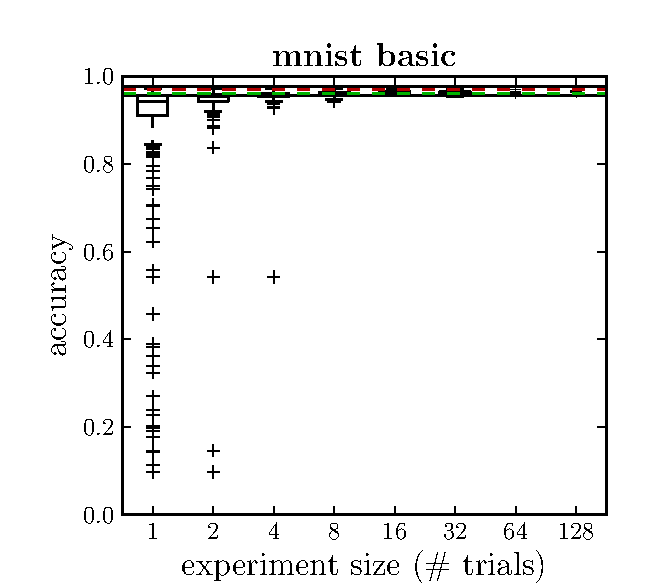
\includegraphics[scale=0.3]{../nips2011paper/figures/dbn_efficiency/dbn_efficiency_mnist_basic}
    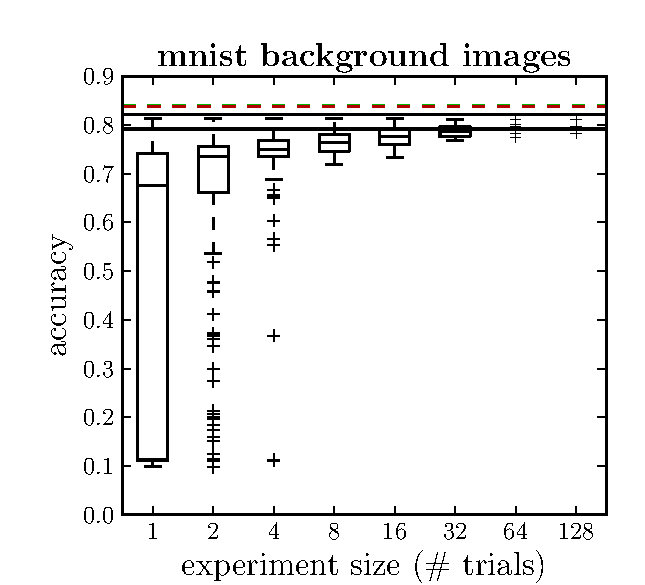
\includegraphics[scale=0.3]{../nips2011paper/figures/dbn_efficiency/dbn_efficiency_mnist_background_images}
    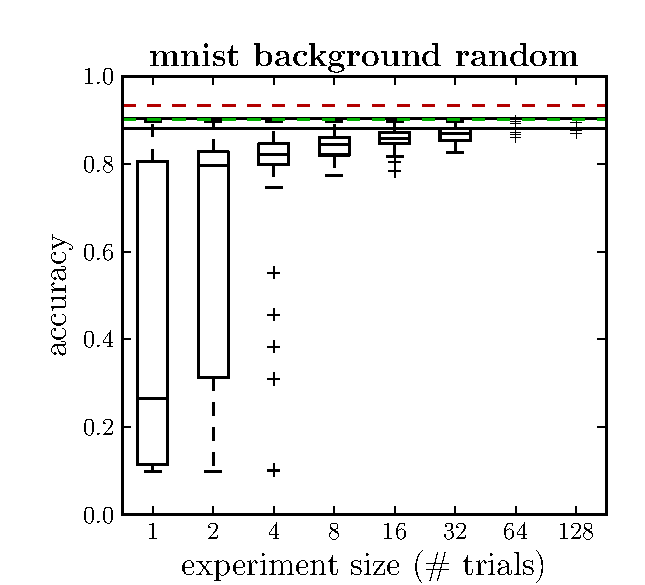
\includegraphics[scale=0.3]{../nips2011paper/figures/dbn_efficiency/dbn_efficiency_mnist_background_random}
    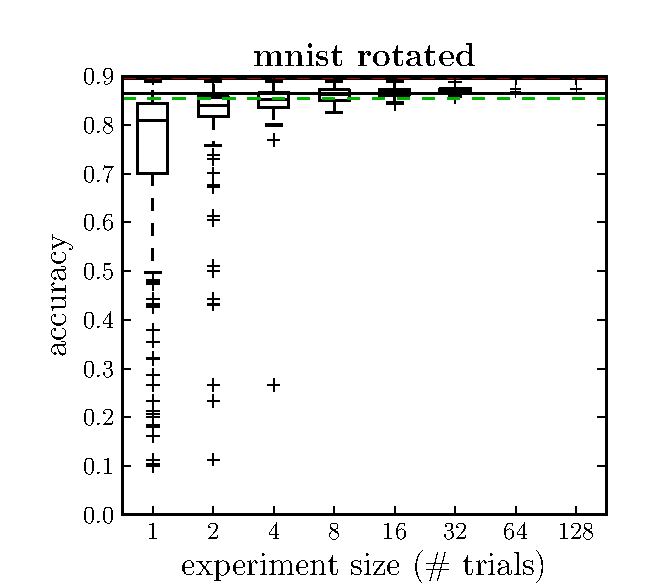
\includegraphics[scale=0.3]{../nips2011paper/figures/dbn_efficiency/dbn_efficiency_mnist_rotated}
    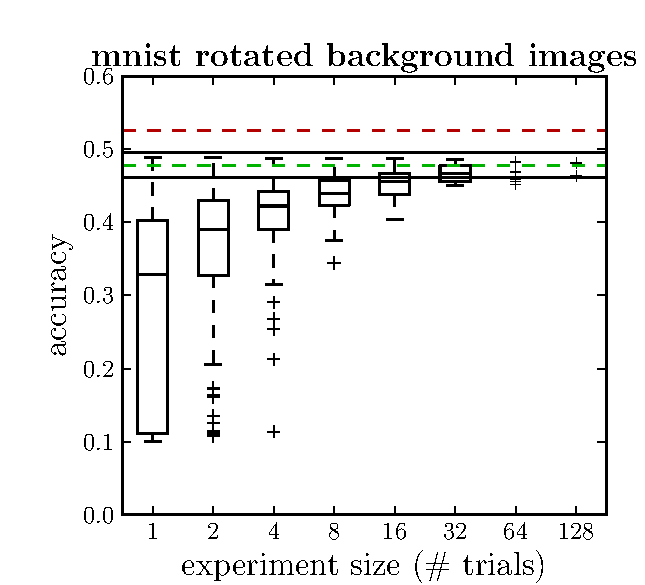
\includegraphics[scale=0.3]{../nips2011paper/figures/dbn_efficiency/dbn_efficiency_mnist_rotated_background_images}
    %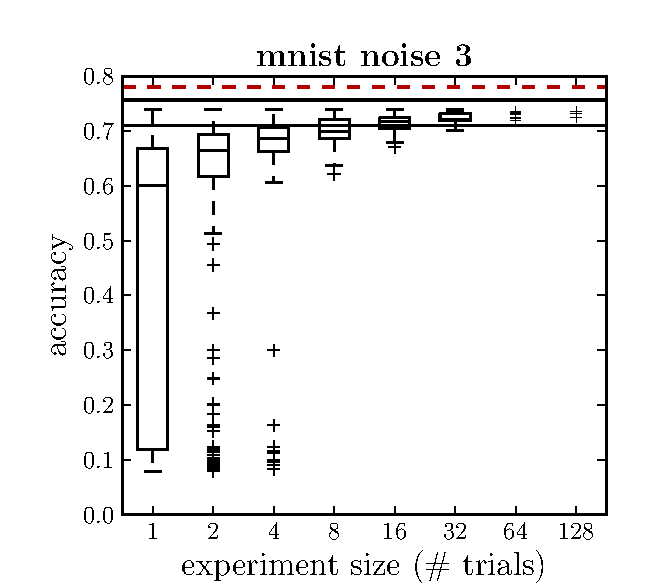
\includegraphics[scale=0.3]{figures/dbn_efficiency/dbn_efficiency_mnist_noise_3}
    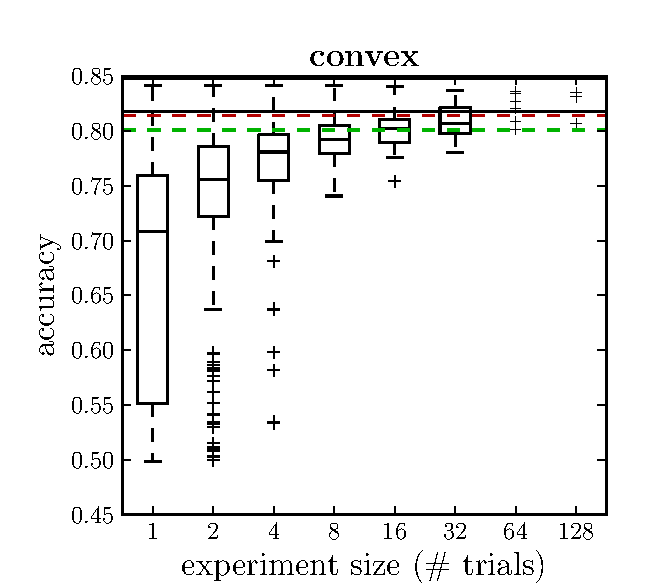
\includegraphics[scale=0.3]{../nips2011paper/figures/dbn_efficiency/dbn_efficiency_convex}
    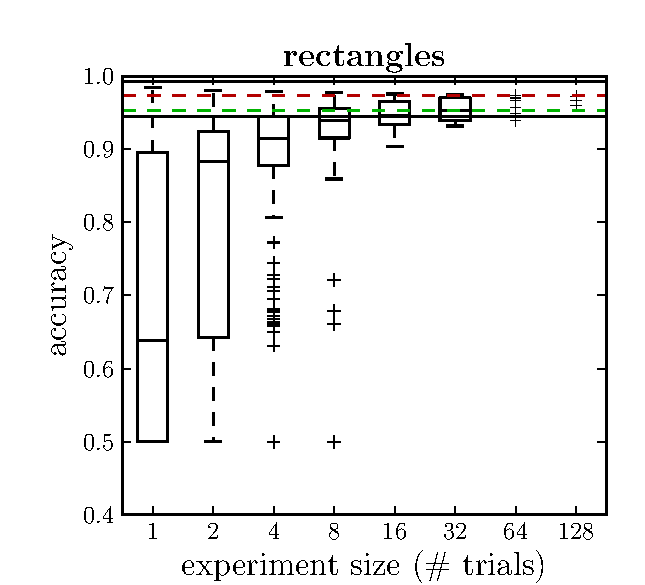
\includegraphics[scale=0.3]{../nips2011paper/figures/dbn_efficiency/dbn_efficiency_rectangles}
    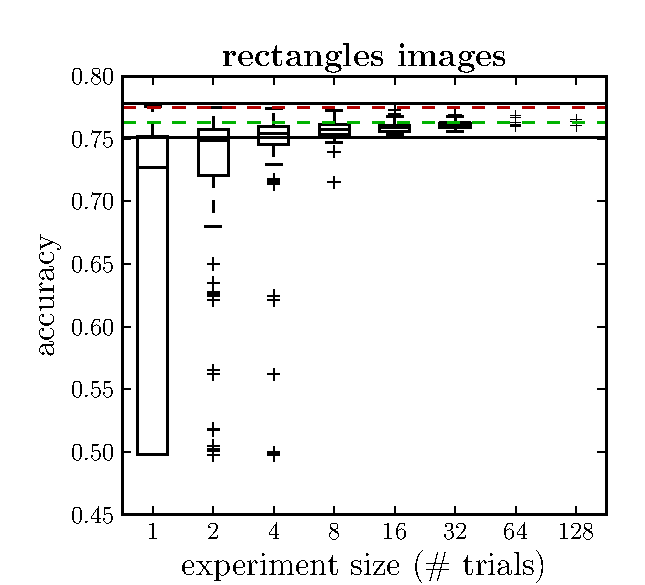
\includegraphics[scale=0.3]{../nips2011paper/figures/dbn_efficiency/dbn_efficiency_rectangles_images}
\vs{2}
    \caption
    {Deep Belief Network (DBN) performance according to random search.
    Random search is used to explore up to 32 hyper-parameters (see Table~\ref{tbl:dbnprior}).
    Results found using a grid-search-assisted manual search over a similar domain with
    an average 41 trials are given in green (1-layer DBN) and red (3-layer DBN).
    Each box-plot (for $N=1,2,4,...)$ shows the distribution of test set performance when the best model among
    $N$ random trials is selected.
    }
    \label{fig:dbn_random_efficiency}
\vs{3}
\end{figure}

